\chapter{Detailed Design}
\label{chap:7}

\section{Class Design}
\label{sec:7.1}

\begin{figure}[htbp]
\centering
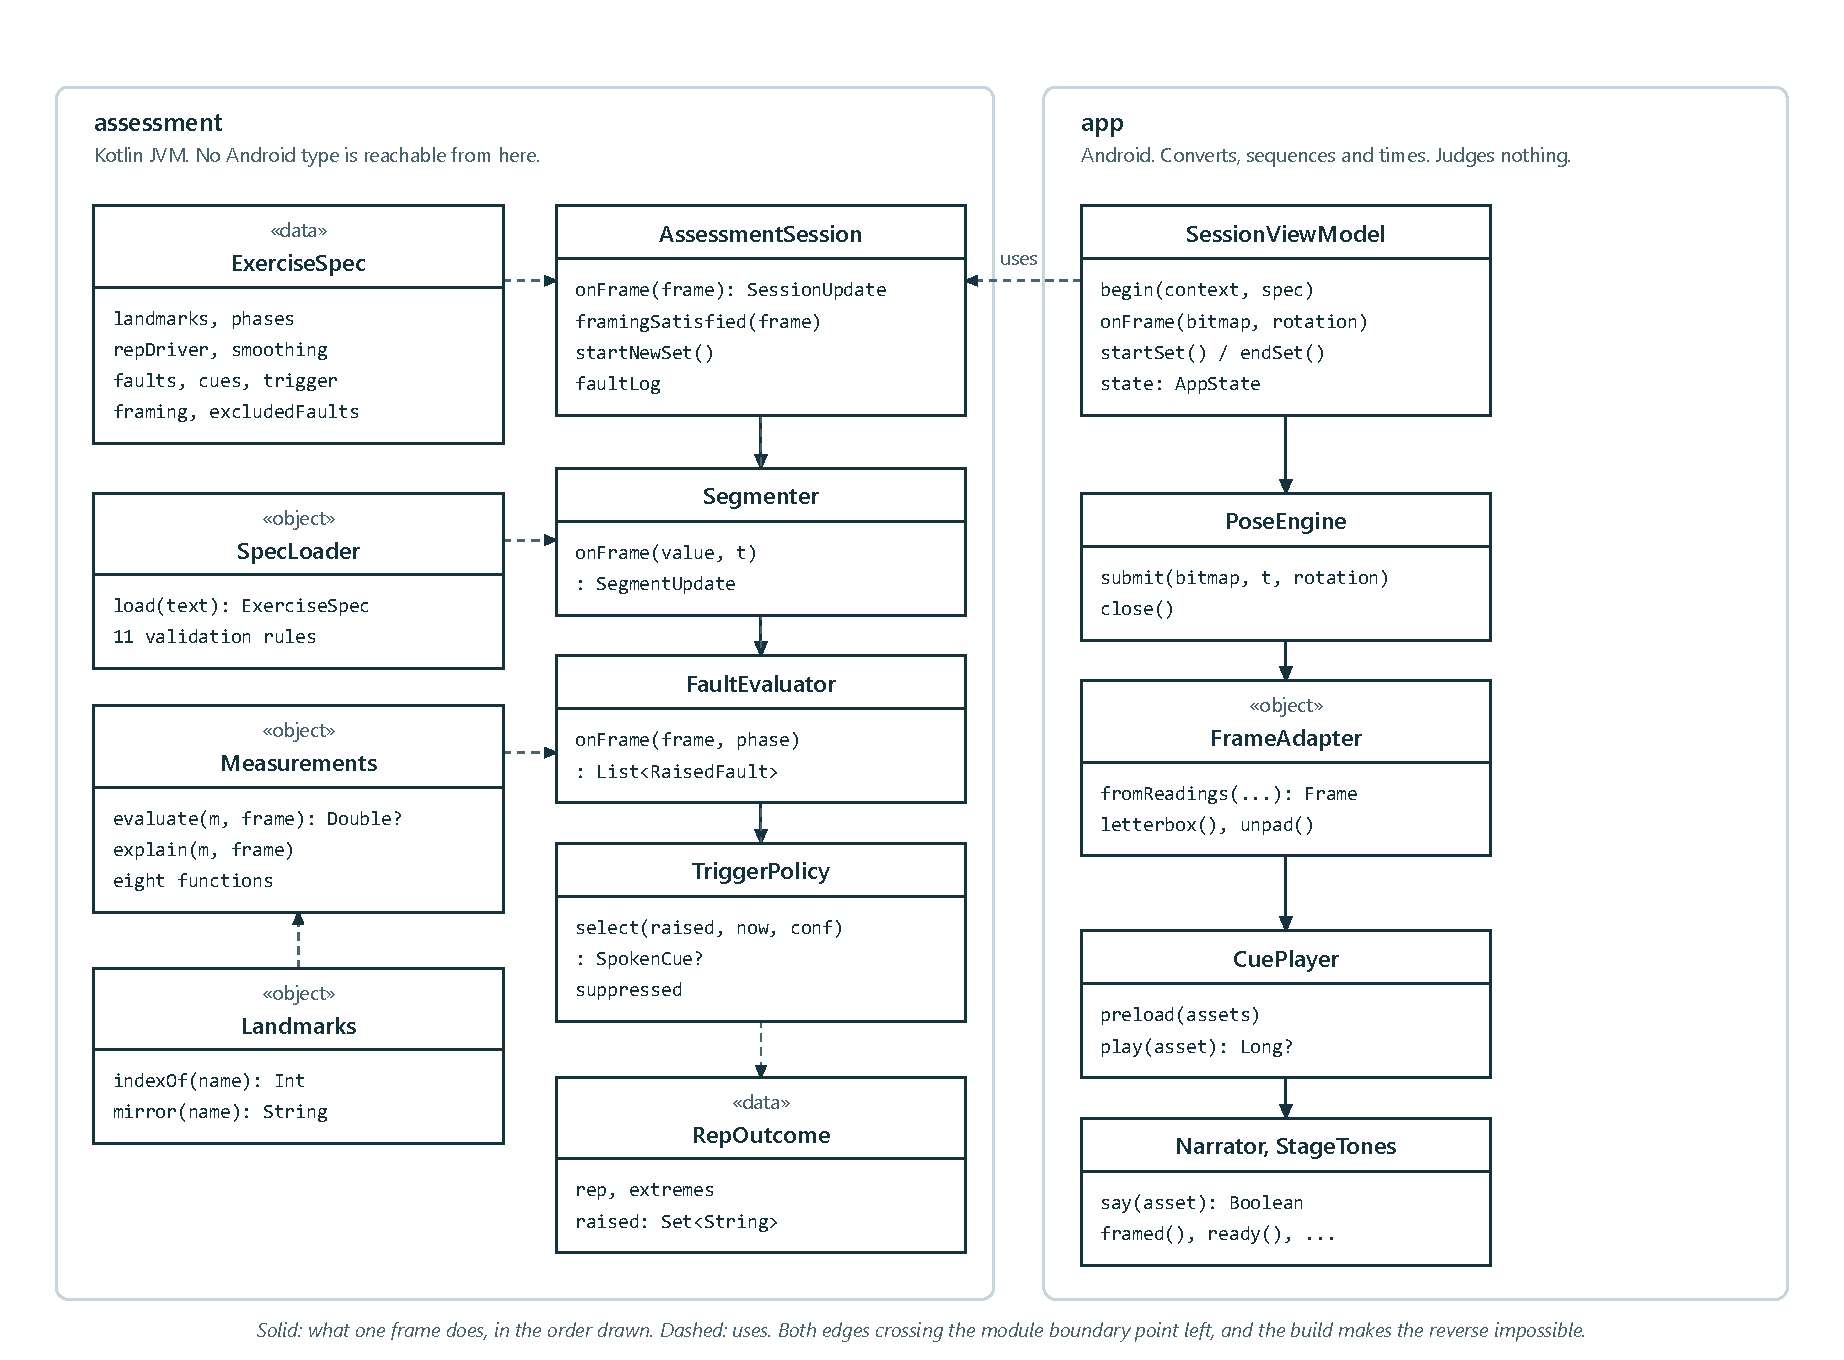
\includegraphics[width=\textwidth]{fig-7-1-classes.pdf}
\caption[The types in the two modules, and the single dependency between them]{The two modules, with every dependency between them pointing in one direction. Nothing on the left can name a type on the right.}
\label{fig:7.1}
\end{figure}

The left column is the assessment module, which is plain Kotlin. The right column is the Android client. There is one edge between them and it points leftward, from the client to the library.

\textbf{The specification, as loaded.}

{\small
\setlength{\LTpre}{6pt}\setlength{\LTpost}{8pt}
\begin{longtable}{>{\raggedright\arraybackslash}p{\dimexpr 0.206\textwidth-2\tabcolsep\relax}>{\raggedright\arraybackslash}p{\dimexpr 0.794\textwidth-2\tabcolsep\relax}}
\caption{The specification as loaded}\\
\toprule
Type & Role \\
\midrule
\endfirsthead
\toprule
Type & Role \\
\midrule
\endhead
\bottomrule
\endfoot
\bottomrule
\endlastfoot
\texttt{Exercise\allowbreak{}Spec} & The parsed file. Landmarks, framing, driver, phases, faults, cues, trigger, exclusions \\
\texttt{Spec\allowbreak{}Loader} & Parses and validates. Eleven rules, each failing with the rule named \\
\texttt{Landmarks} & Name to index, and the mirror of a name. The only type that knows the engine's layout \\
\texttt{Measurements} & The eight measurement functions, and the normalisers \\
\end{longtable}
}

\textbf{The live assessment.}

{\small
\setlength{\LTpre}{6pt}\setlength{\LTpost}{8pt}
\begin{longtable}{>{\raggedright\arraybackslash}p{\dimexpr 0.285\textwidth-2\tabcolsep\relax}>{\raggedright\arraybackslash}p{\dimexpr 0.715\textwidth-2\tabcolsep\relax}}
\caption{The live assessment}\\
\toprule
Type & Role \\
\midrule
\endfirsthead
\toprule
Type & Role \\
\midrule
\endhead
\bottomrule
\endfoot
\bottomrule
\endlastfoot
\texttt{Assessment\allowbreak{}Session} & The one object the client talks to. Takes a frame, returns a \texttt{Session\allowbreak{}Update} \\
\texttt{Segmenter} & Driver, smoothing, hysteresis, phases, counts and hold duration \\
\texttt{Fault\allowbreak{}Evaluator} & Continuous faults: the streak over the declared phases \\
\texttt{Trigger\allowbreak{}Policy} & Which raised fault, if any, becomes a cue \\
\texttt{Rep\allowbreak{}Outcome} & What one repetition came to, emitted at every closing boundary \\
\end{longtable}
}

\textbf{The client.}

{\small
\setlength{\LTpre}{6pt}\setlength{\LTpost}{8pt}
\begin{longtable}{>{\raggedright\arraybackslash}p{\dimexpr 0.480\textwidth-2\tabcolsep\relax}>{\raggedright\arraybackslash}p{\dimexpr 0.520\textwidth-2\tabcolsep\relax}}
\caption{The client}\\
\toprule
Type & Role \\
\midrule
\endfirsthead
\toprule
Type & Role \\
\midrule
\endhead
\bottomrule
\endfoot
\bottomrule
\endlastfoot
\texttt{Session\allowbreak{}View\allowbreak{}Model} & Sequences a session and holds the state the interface renders \\
\texttt{Pose\allowbreak{}Engine} & Loads the model, runs inference, drops a frame that arrives while busy \\
\texttt{Frame\allowbreak{}Adapter} & Letterbox and un-pad, presence floor, tensor to named landmarks \\
\texttt{Cue\allowbreak{}Player}, \texttt{Narrator}, \texttt{Stage\allowbreak{}Tones} & Audio: the fault cues, the spoken stages, the non-verbal markers \\
\end{longtable}
}

Two aspects of the arrangement carry most of its value.

\textbf{\texttt{Assessment\allowbreak{}Session} is the only entry point.} The client does not reach into the segmenter or the evaluator. It calls \texttt{on\allowbreak{}Frame} and receives a phase, a count, the raised faults, and at most one cue. This is what makes the assessment layer replaceable in one place, and it is what the offline replay harness substitutes for.

\textbf{\texttt{Landmarks} is the only type that knows the engine's output layout.} The specifications name landmarks as strings and every measurement resolves them through this one table. Changing the pose engine changed this file and the adapter, and reached no specification and no rule.

\section{Activity Flow}
\label{sec:7.2}

\begin{figure}[htbp]
\centering
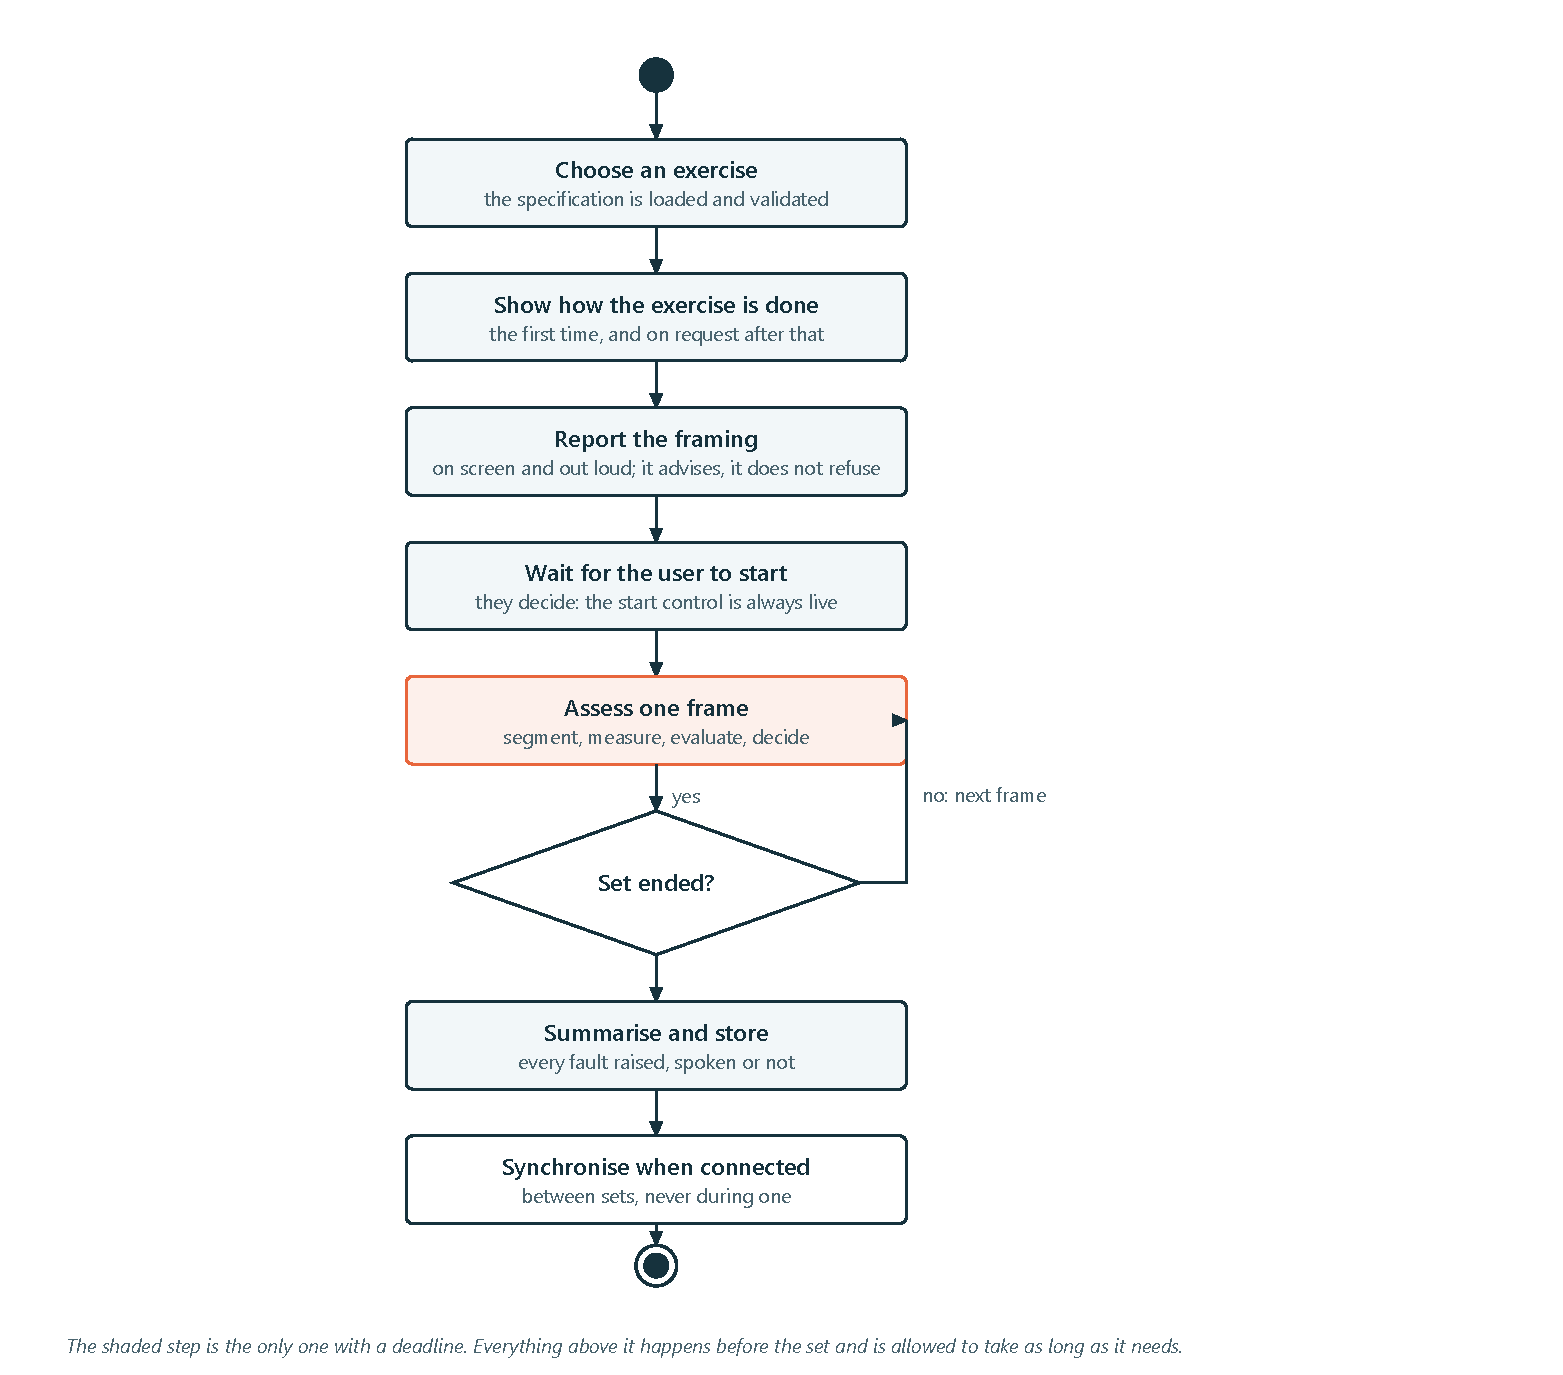
\includegraphics[width=\textwidth]{fig-7-2-session-activity.pdf}
\caption[A session from launch to a written record]{One session. Nothing before the set can send the trainee backwards; the only loop is the frame loop.}
\label{fig:7.2}
\end{figure}

The flow has no gate in it. Before the set the system does two things and blocks on neither: it shows how the exercise is performed, and it reports the framing conditions in the specification, which are the required landmarks visible above the floor and the body occupying a usable part of the frame. When a condition fails the system names the correction needed on screen and goes on naming it. Starting remains one tap throughout. Nothing is spoken before the set except the line confirming it has started: the correction is the same sentence the guide already shows, and a product that reads its own screen aloud while the trainee is standing at it has misread who is where.

An earlier design refused to start until the framing passed. What defeats it is the physical loop: the trainee presses start at the phone and then walks into position, so the framing a pre-set gate measures is the framing of somebody standing beside the camera. The gate was close to free of information and it cost the product the posture of deciding whether a person may train. What the condition genuinely bounds is what the assessment can see, and that is handled where it bites: an unmeasurable landmark makes the faults that need it unmeasured for those frames, which the record states, and the set summary reports what was and was not seen.

Once the set starts it runs without interaction. The trainee's hands are occupied and the screen faces away from them, so everything between the start and the end of a set is audio, which NFR-U1 and NFR-U2 require.

At the end the system stops the pipeline, writes the record, and shows the summary. The summary is the first thing in the whole flow that assumes the trainee is looking at the screen.

\section{Sequence: One Frame to One Cue}
\label{sec:7.3}

\begin{figure}[htbp]
\centering
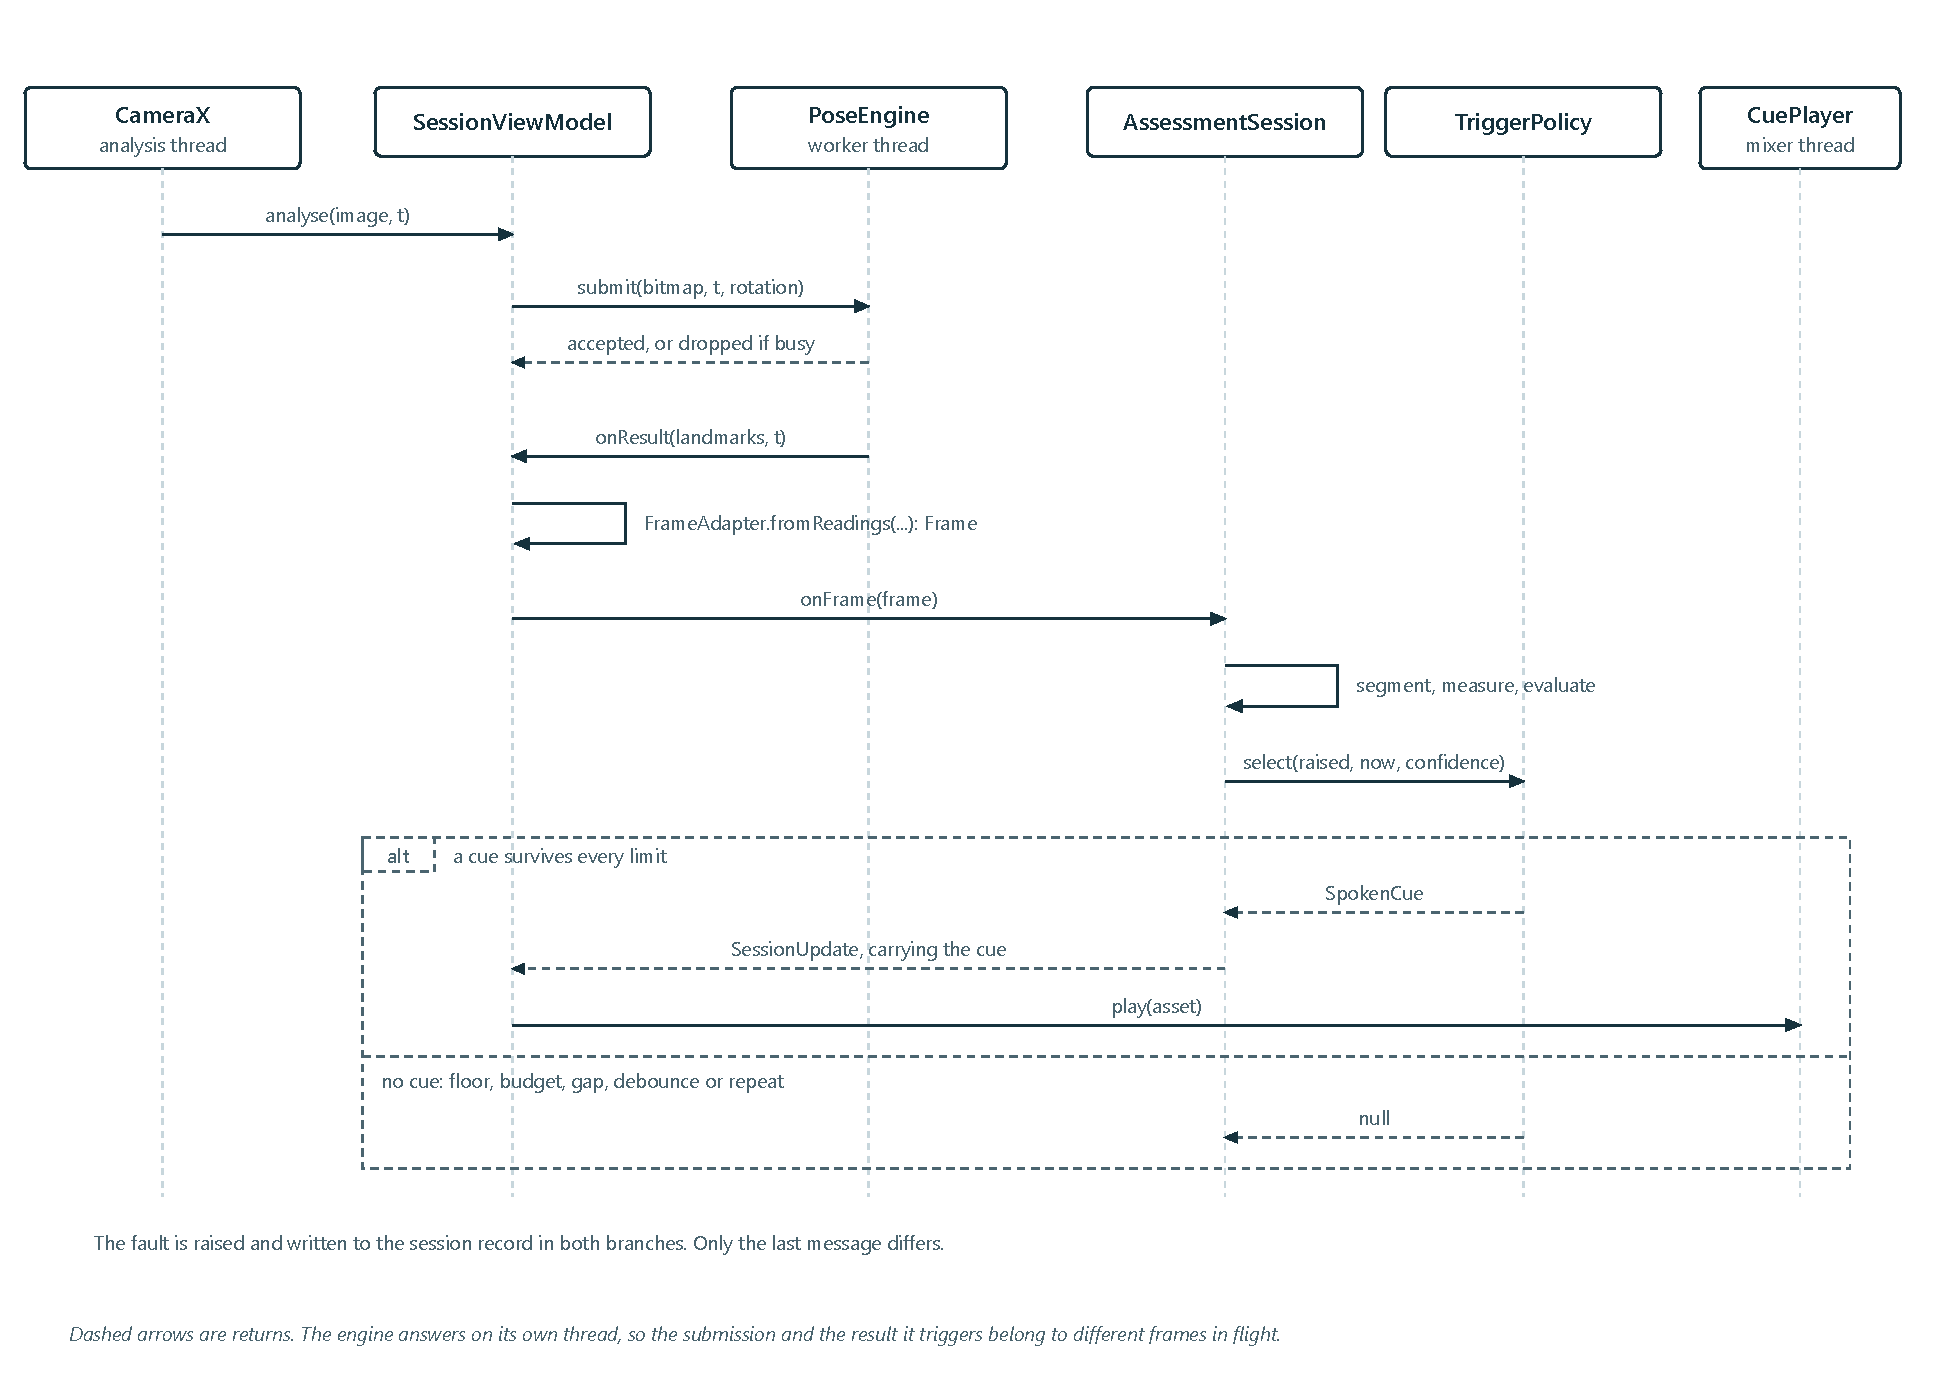
\includegraphics[width=\textwidth]{fig-7-3-frame-to-cue.pdf}
\caption[The call sequence for a single frame, including the paths that end in silence]{One frame. Most frames take one of the early exits.}
\label{fig:7.3}
\end{figure}

The sequence is worth reading for its exits rather than its happy path. A frame can stop at the busy check, at the pose result, at the visibility floor, at the phase scope, at the confirmation streak, at the confidence floor, or at the rate limit. Each is a different reason, and the common case is that a frame stops at one of them.

Three points in the sequence decide the latency the trainee experiences.

\textbf{The timestamp is taken at capture, not at arrival.} Everything downstream measures from when the camera saw the movement rather than from when the application got round to it, so a queueing delay cannot hide inside the figure.

\textbf{The cue is a clip already in memory.} \texttt{Cue\allowbreak{}Player.\allowbreak{}preload} loads every asset the specification names when the session begins, so the path from a confirmed fault to the first audible sample is a map lookup and a play call. There is no file read and no synthesis in it, which is what makes the allocation in 3.4.1 met by construction.

\textbf{The record of what was spoken is taken from the audio layer}, not from the decision to speak. The two differ whenever the policy suppresses, and keeping them separate is what lets a set report six faults raised and two cues spoken without the two numbers contradicting each other.

\section{State Machines}
\label{sec:7.4}

\begin{figure}[htbp]
\centering
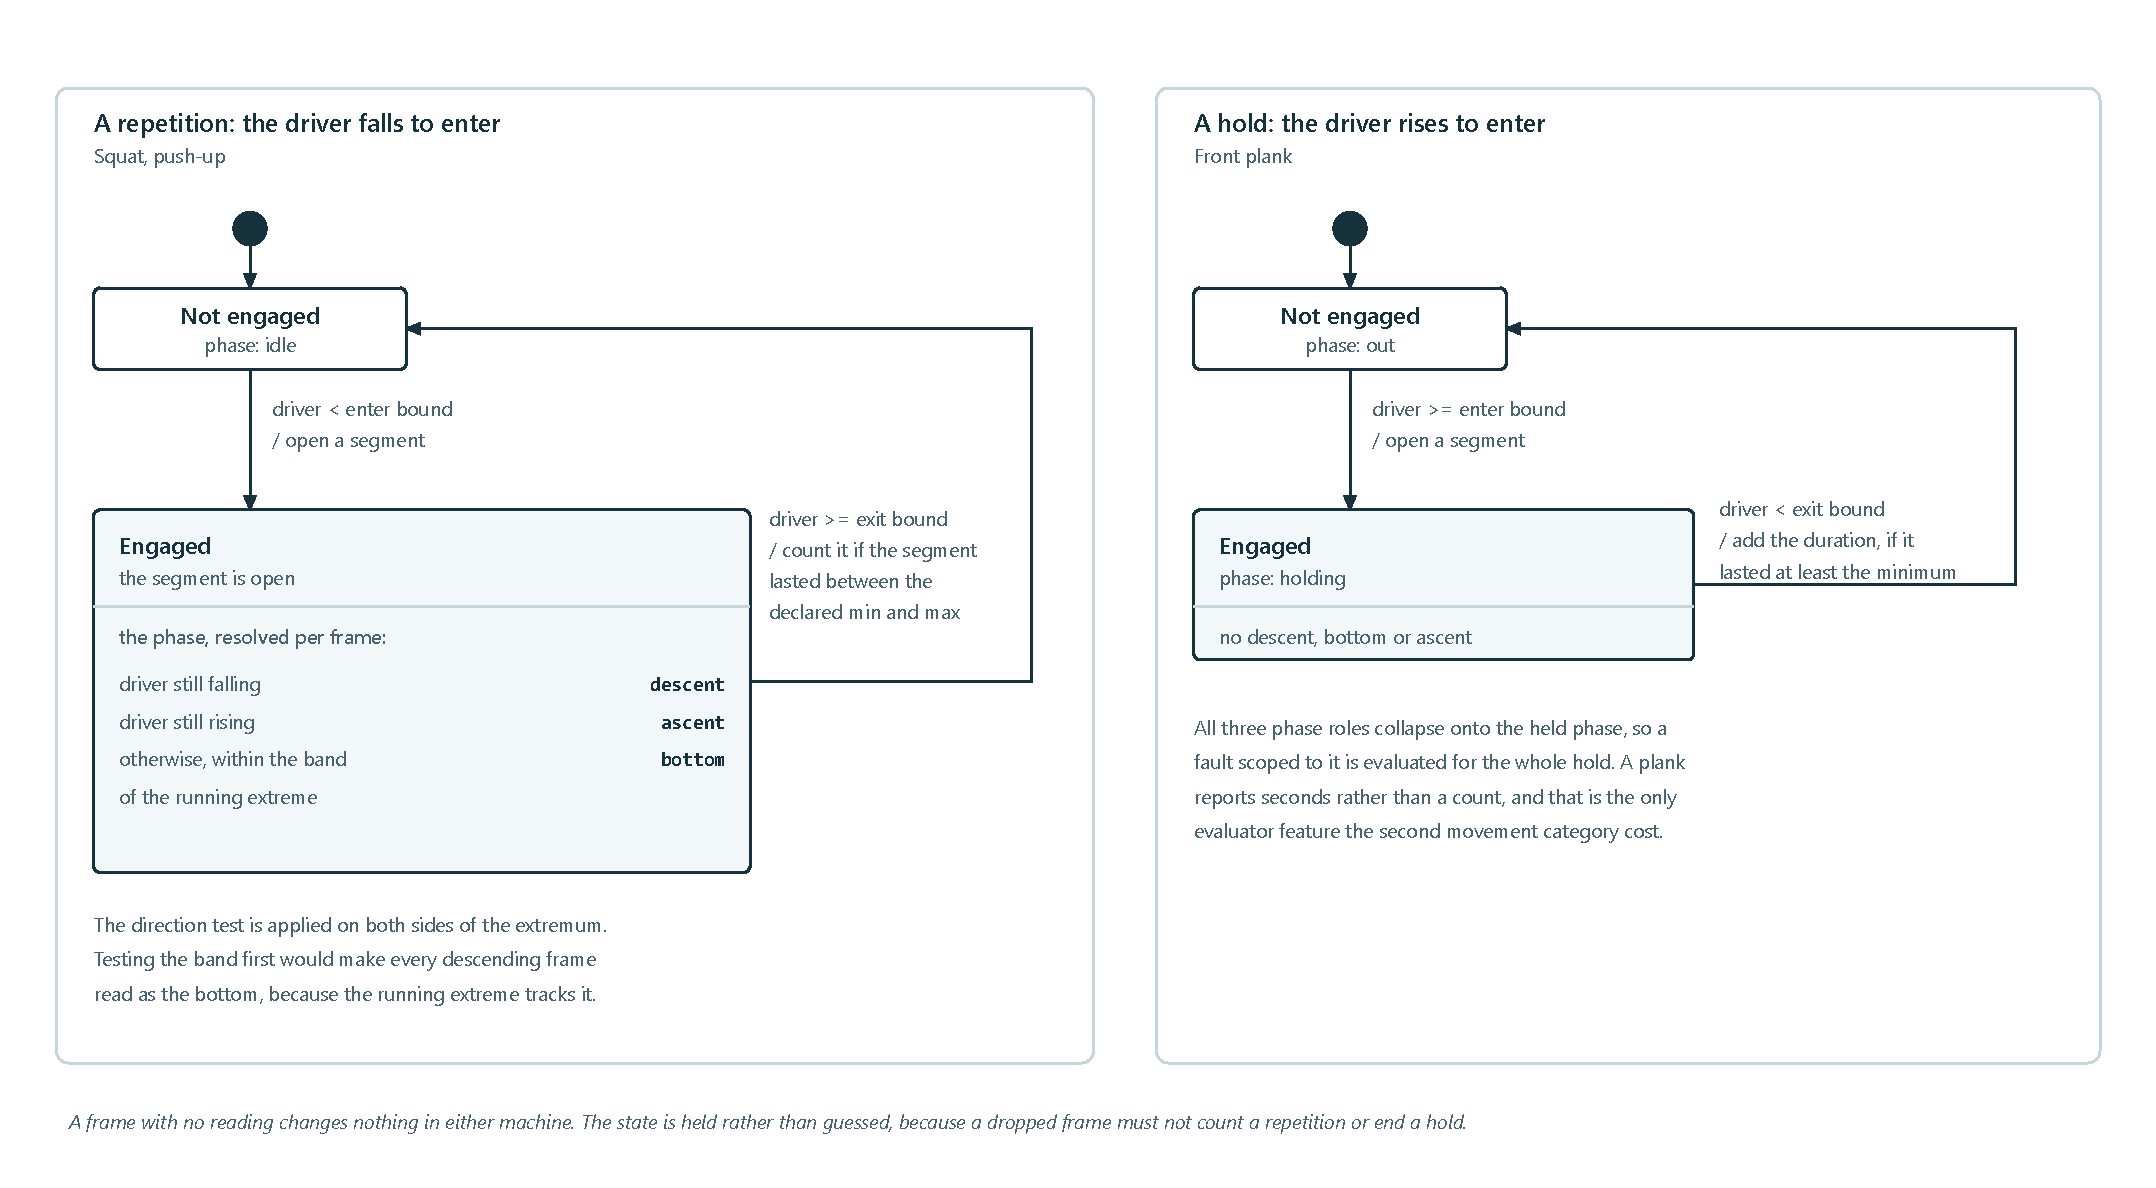
\includegraphics[width=\textwidth]{fig-7-4-segmenters.pdf}
\caption[The counting segmenter and the hold segmenter, side by side]{The same machine twice. Only the entry comparison and what is reported at the end differ.}
\label{fig:7.4}
\end{figure}

The segmenter is one state machine with two configurations.

\textbf{Counting.} Idle until the driver falls below the entry bound; engaged until it rises past the completion bound. On completion, the elapsed time is checked against the declared bounds and the count advances if it passes. Within the engaged state the phase is resolved from the direction of travel: falling is the descent, rising is the ascent, and a driver that has stopped moving within a band of its own extreme is the bottom.

\textbf{Holding.} The same machine with the entry comparison reversed. Entered when the driver rises past its bound, left when it falls back under the other, and the time accumulated rather than counted.

Three details in the implementation are worth naming.

\textbf{Stillness is tested against the measurement's own noise.} The bottom phase is where the driver has stopped moving, which requires a threshold for what counts as movement. That threshold has to sit above the frame-to-frame noise of the pose estimate or the phase is never entered at all. It is a property of the engine rather than of the movement, and 4.2.5 records what happened when it was carried across an engine change unchanged.

\textbf{An unmeasurable driver does not reset the machine.} At the bottom of a squat the ankle can leave the frame, and the driver stops resolving. The segmenter holds its state and reports the phase it was in, rather than treating a missing measurement as a return to idle. This is why the per repetition evaluation mode samples every engaged frame instead of the frames at the driver's extreme.

\textbf{The duration bounds are applied at the close, not during.} A segment is only rejected once its length is known, so a trainee pausing mid-repetition is not cut off partway through; the repetition simply does not count when it ends.

\subsection{The declared phase conditions are not parsed}
\label{sec:7.4.1}

The specification describes each phase in prose: the bottom is \textit{``driver at local minimum, within 10 degrees of it''}. The evaluator does not parse that sentence. The band is a constant in the segmenter, and the phase names in the file are matched to roles by position.

This is a real gap between what the format appears to declare and what the evaluator reads, and it is recorded rather than closed. The effect is bounded: a new exercise in either supported category gets the same phase behaviour as the existing ones whatever its prose says, and an exercise needing different phase semantics needs an evaluator change and not only a file.

It is stated here because a reviewer reading the specification would otherwise reasonably believe the sentence was executable.

\section{Data Model}
\label{sec:7.5}

One record per set, written locally when the set ends.

{\small
\setlength{\LTpre}{6pt}\setlength{\LTpost}{8pt}
\begin{longtable}{>{\raggedright\arraybackslash}p{\dimexpr 0.413\textwidth-2\tabcolsep\relax}>{\raggedright\arraybackslash}p{\dimexpr 0.587\textwidth-2\tabcolsep\relax}}
\caption{The set record written when a set ends}\\
\toprule
Field & Contents \\
\midrule
\endfirsthead
\toprule
Field & Contents \\
\midrule
\endhead
\bottomrule
\endfoot
\bottomrule
\endlastfoot
\texttt{exercise}, \texttt{spec\_\allowbreak{}id}, \texttt{spec\_\allowbreak{}version} & Which exercise, and the version of the file in force \\
\texttt{started\_\allowbreak{}at}, \texttt{ended\_\allowbreak{}at}, \texttt{duration\_\allowbreak{}s} & When the set ran, and how long it took \\
\texttt{reps} or \texttt{hold\_\allowbreak{}s} & The result, by the exercise's declared scoring mode \\
\texttt{reps\_\allowbreak{}with\_\allowbreak{}fault} & How many repetitions carried any fault \\
\texttt{faults}, \texttt{cues} & Every fault raised, and every cue actually spoken, each with its timing \\
\texttt{reps\_\allowbreak{}detail} & One row per repetition: its number, the measured value behind each per-repetition fault, and what was raised \\
\texttt{cues\_\allowbreak{}spoken} & How many the trainee actually heard \\
\texttt{suppressed} & Why a raised fault did not become a cue, counted by reason \\
\texttt{measured} & Per fault, the range of values seen and how many frames were measurable \\
\texttt{pose\_\allowbreak{}rate}, \texttt{fps} & The coverage behind the whole record \\
\end{longtable}
}

\textbf{\texttt{spec\_\allowbreak{}version} is what makes an old record readable.} A fault code means what the specification of that version said it meant. A record without its version becomes uninterpretable the first time a threshold moves, and thresholds in this project have moved.

\textbf{\texttt{reps\_\allowbreak{}detail} stores the value for every repetition, including the ones that passed.} A count of faults answers how many and not which, and it cannot distinguish a set of repetitions that were comfortably correct from a set that passed by a hair. The per-repetition value is what makes a later reader able to tell those apart, and it is what the evaluation in 9.4 is computed from.

\textbf{\texttt{pose\_\allowbreak{}rate} is kept because it qualifies everything else.} A set in which the engine lost the body for a quarter of its frames has a repetition count and a fault count that mean less than the same numbers from a set with full coverage. Storing it means the qualification travels with the record instead of being lost. \texttt{suppressed} and \texttt{measured} are there for the same reason from the other direction: a quiet set and a set that detected nothing look identical without them.

Records are held in application-private storage. Nothing else about a session is written: no frame, no still image and no landmark sequence. That is what NFR-S1 asserts, and a reader can check it by looking for a write path and finding none.
